\chapter{Opis projektnog zadatka}
		
		\textbf{\textit{dio 1. revizije}}\\
		
		\textit{Na osnovi projektnog zadatka detaljno opisati korisničke zahtjeve. Što jasnije opisati cilj projektnog zadatka, razraditi problematiku zadatka, dodati nove aspekte problema i potencijalnih rješenja. Očekuje se minimalno 3, a poželjno 4-5 stranica opisa.	Teme koje treba dodatno razraditi u ovom poglavlju su:}
		\begin{packed_item}
			\item \textit{potencijalna korist ovog projekta}
			\item \textit{postojeća slična rješenja (istražiti i ukratko opisati razlike u odnosu na zadani zadatak). Dodajte slike koja predočavaju slična rješenja.}
			\item \textit{skup korisnika koji bi mogao biti zainteresiran za ostvareno rješenje.}
			\item \textit{mogućnost prilagodbe rješenja }
			\item \textit{opseg projektnog zadatka}
			\item \textit{moguće nadogradnje projektnog zadatka}
		\end{packed_item}
		
		\textit{Za pomoć pogledati reference navedene u poglavlju „Popis literature“, a po potrebi konzultirati sadržaj na internetu koji nudi dobre smjernice u tom pogledu.}\\
		
		\textnormal{Cilj projekta grupe PI je razviti programsku podršku za stvaranje web aplikacije "GeoFighter".  GeoFighter je igra u kojoj se igrači međusobno bore kartama koje su sakupili na različitim stvarnim lokacijama. Cilj igrača je postići što veći rang na globalnoj ljestvici dok je njihov zadatak obići što više  gradova, naselja, planina, umjetničkih instalacija, znamenitosti i slično te sakupiti iste. Lokacije su u obliku igraćih karata. Svaka karta ima naziv,  opis, fotografiju i oznaku 3 atributa. Igrači s 10 ili više pobjeda imaju opciju prijaviti željenu lokaciju pored koje se nalaze. U prijavi lokacije igrači su dužni navesti ime lokacije i opis, dok jačinu karte određuje kartograf. \\\\ \underline{Kartograf} je osoba koja je zadužena za nadopunjavanje baze podataka s lokacijama koje su igrači prijavili. On ih može odbiti, potvrditi, urediti ili označiti da je potrebna potvrda s terena. Ukoliko kartograf prihvati lokaciju bez izmjena, igrač koji je lokaciju  prijavio dobiva tu kartu.}\\
		
		\textnormal{\underline{Administrator} ima najveće ovlasti. Uz ovlasti igrača i kartografa administrator može vidjeti i uređivati popis svih korisnika i njihovih osobnih  podataka. On može dodijeliti  igračima i privremeno isključenje iz igre. Dodatno može uređivati i postojeće lokacije u igri.}
		
		\textnormal{Registriranom korisniku omogućena je prijava u sustav s postojećim računom, dok neregistrirani korisnici imaju mogućnost kreiranja novog računa.}
		
		\textnormal{Za kreiranje korisničkog računa igrača potrebno je:}
		\begin{packed_item}
			\item \textbf{korisničko ime}
			\item \textbf{fotografija}
			\item \textbf{email adresa}
			\item \textbf{lozinka}
		\end{packed_item}
		\textit{Nakon  popunjavanja  podataka,  na njegovu email adresu se šalje link kojim može potvrditi svoj račun.}
		
		\textnormal{Za kreiranje korisničkog računa kartografa potrebno je:}
		\begin{packed_item}
			\item \textbf{broj IBAN računa}
			\item \textbf{fotografija osobne iskaznice}
		\end{packed_item}
		\textit{Kartografa potvrđuje administrator.}
		
		\textbf{\underline{Nakon kreiranja računa igrača}}
		\begin{figure}[H]
			\centering
			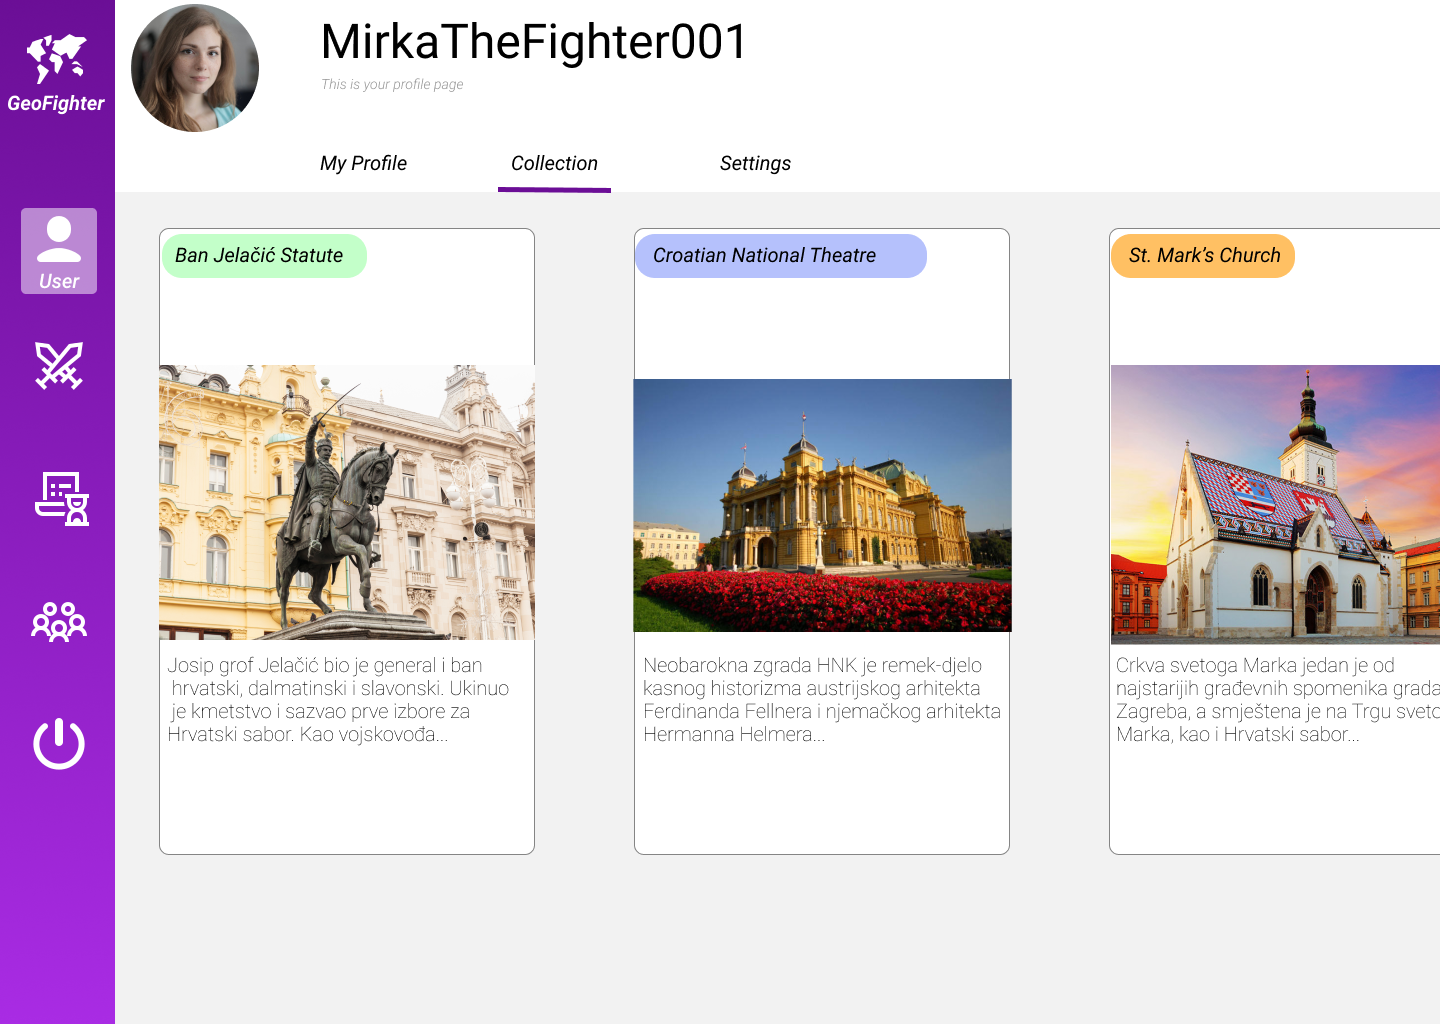
\includegraphics[scale=0.2]{slike/example} \\%veličina u odnosu na širinu linije
			\caption{WorkInProgress Primjer UI igrača}
			\label{fig:example} %label mora biti drugaciji za svaku sliku
		\end{figure}
	
	
		\textnormal{Igračima je dostupan pregled profila igrača, globalna statistika odigranih borbi i sakupljenih lokacija te poredak svih igrača prema elo sustavu. Prilikom pregleda profila nekog igrača, prikazuju se sve karte koje je igrač ikad sakupio, rang na globalnoj ljestvici i statistike vezane uz zadnjih 10 borbi s drugim igračima. Istražujući svoju okolinu igrači sakupljaju lokacije tako da im dođu na dovoljnu udaljenost (~1km). Lokacije se sakupljaju u obliku igraćih karata koje igrači koriste za međusobne bitke. Pritiskom na gumb ukriženih mačeva, igrač pristupa popisu igrača koji se nalaze u radijusu 50km od njega. Ukoliko igrač želi započeti bitku pritiskom na ime drugog igrača šalje zahtjev za borbu. Nakon 10 osvojenih borbi igraču se otvara opcija da sam pridonosi bazi podataka GeoFighter-a tako da prijavljuje lokacije sa slikom, nazivom i opisom te lokacije.}\\
	
		\textnormal{Igrač može vidjeti popis ostalih aktivnih igrača koji se nalaze unutar 50km i s njima ući u borbu. Borba se sastoji od 5 rundi. Svaka karta ima 3 atributa u vrijednosti 0-100 (0-najslabije, 100-najjače). Borba započinje bacanjem novčića koji odlučuje koji će igrač imati prvi potez. Igrač koji je pobijedio bacanje novčića započinje bitku bacanjem karte i odabirom jednog od tri atributa s karte. Protivnik baca svoju kartu te se gleda čija karta ima jači zadani atribut. Igrač koji je pobijedio trenutnu rundu započinje iduću rundu sve dok se ne odigra svih 5 rundi. Rating se dodjeljuje prema ELO ratingu koji se koristi u šahu.}
		\textnormal{Nakon borbe, korištene karte ne mogu se koristiti 72 sata kako bi se igrače potaknulo na aktivan život i istraživanje.}\\
		
		\textnormal{Sučelje kartografa razlikuje se od sučelja igrača. Kartografu se prijave pokazuju na karti te ukoliko nije zadovoljan prijavom i/ili želi provjeriti danu lokaciju, sustav preko vanjskog servisa OSRM(Open source routing machine) dohvati rješenje problema trgovačkog putnika i kartografu put prikaže na karti. Nakon analize prijave, kartograf odlučuje hoće li prijavu odbiti nepovratno, prihvatiti prijavu i dodijeliti 3 atributa lokaciji te ju tako pretvoriti u igraću kartu, prepraviti prijavu nakon provjere na terenu (promjena slike ili opisa) i dodijeliti 3 atributa lokaciji ili će označiti prijavu kao nepotpunu te uz komentar "vratiti" prijavu igraču na doradu. Ukoliko je kartograf prihvatio prijavu bez dorada, igraču se dodjeljuje igraća karta te lokacije.}\\
		
		\textnormal{Sučelje administratora sastoji se od sučelja igrača, kartografa te sučelja administratora. Prebacivanjem (toggle button) sučelja administrator bira želi li igrati kao igrač, raditi kao kartograf ili želi obavljati posao administratora. Administrator može pritiskom na gumb vidjeti popis svih registriranih igrača i kartografa, vidjeti i mijenjati njihove osobne podatke. On jedini može brisati i uređivati postojeće lokacije tj. igraće karte.}\\
		
		
		\textnormal{Ovaj projekt potencijalno bi mogao koristiti korisnicima različitih generacija i interesa. Igra će biti izvrsno rješenje za djecu koja više vole igrati igrice nego provoditi vrijeme na otvorenom. Osim što će mlađe generacije izaći van na svjež zrak, baviti se tjelesnom aktivnošću i pritom igrati omiljenu im igricu, zajedno s prijateljima otkrivat će znamenitosti i ljepote Hrvatske te ponešto o svakoj naučiti.}
		
		\textnormal{Projekt će biti novi izazov za svakog gamera, malo drugačiji pogled na web-igre i razlog zbog kojeg će se mnoge korisnike redovno poticati na tjelesnu aktivnost. Promicat će se kulturna baština, širiti opće znanje stanovnika Republike Hrvatske, odlaziti u slabije pojećivana mjesta, a ovaj projekt mogao bi pozitivno pridonijeti i turizmu. Za turiste koji nisu u žurbi igra će biti savršen način za upoznavanje grada i istraživanje zanimljivih lokacija.}\\
		
		
		\textnormal{Najpoznatije postojeće slično rješenje je igra za ručne mobilne uređaje \textbf{Pokémon GO}. Pomoću GPS lokacije igrača oni se smještaju na virtualnu mapu koja emulira stvarni svijet, uz dodane lokacije gdje je moguća borba i sakupljanje Pokémona koji služe za borbu. Borbe se odvijaju pomoću jačine Pokémona, kao što će to biti slučaj s kartama u ovome projektu. Razlike u odnosu na ovaj projekt su to što je u igrici Pokémon GO omogućen prikaz mape po kojoj se igrač kreće analogno svom kretanju u stvarnosti te što će u našem projektu označene lokacije biti važne za sakupljanje igraćih karata, no ne i za samo održavanje borbe. Za održavanje borbi u našem projektu će biti samo važni igrači koji su udaljeni 50 km od korisnika kako bi se pronašao suigrač, ali ne i sama lokacija korisnika kao što je to u Pokémon GO.    }
		
		\begin{figure}[H]
			\centering
			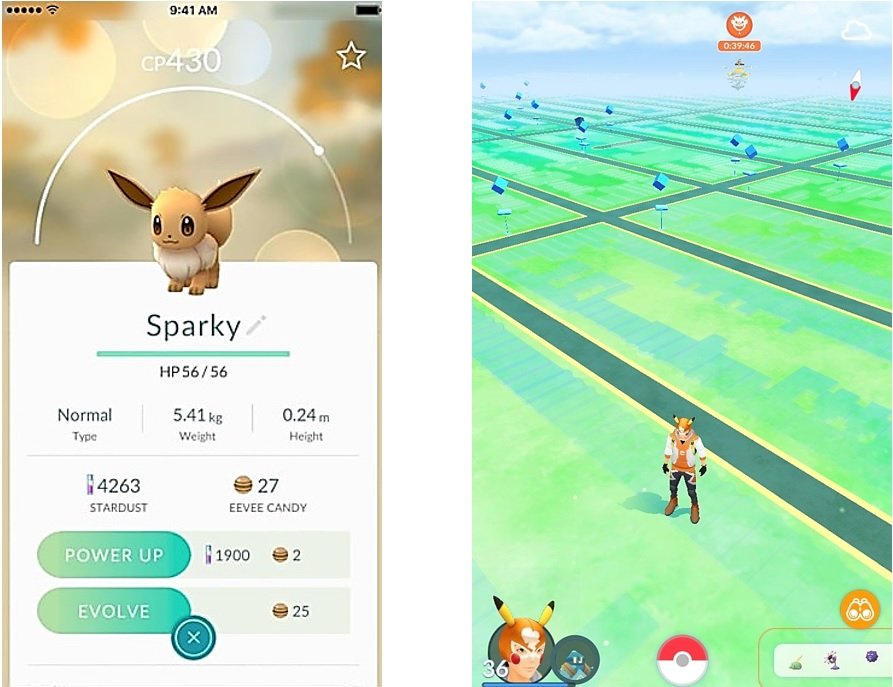
\includegraphics[scale=0.45]{slike/PokemonGO} \\%veličina u odnosu na širinu linije
			\caption{Prikaz kartice Pokémona i mape igrice Pokémon GO}
			\label{fig:PokemonGO} %label mora biti drugaciji za svaku sliku
		\end{figure}
	
		\textnormal{\textbf{Maguss} je mobilna igrica u kojoj su korisnici pomoću GPS-a smješteni na virtualnu mapu koja emulira stvarni svijet, ali uz dodatne lokacije na kojima je moguće sakupiti razna stvorenja, napitke i čarolije u obliku kartica. Prva razlika je što ovaj projekt neće imati prikaz kretanja po mapi, što je omogućeno u igrici Maguss, te će također postojati samo jedna vrsta stvari koju je moguće sakupiti, točnije kartica lokacije. Koncept duela sličan je borbama u ovome projektu jer se odvija karticama te suparnici ne moraju biti na identičnoj lokaciji, ali je različit po tome što dueli u igrici Maguss uključuju i dodatne zadatke kao što su iscrtavanje poteza. Također, jedna od bitnih razlika ovih igrica je to što se jačina kartica ne mijenja u igrici Maguss kao što je to slučaj u ovome projektu, već se pobjedama mijenja jačina igrača. Za razliku od našeg projekta, kretanje u ovoj igrici osim pronalaska novih kartica djeluje i kao način punjenja energije igrača.   }
		
		\begin{figure}[H]
			\centering
			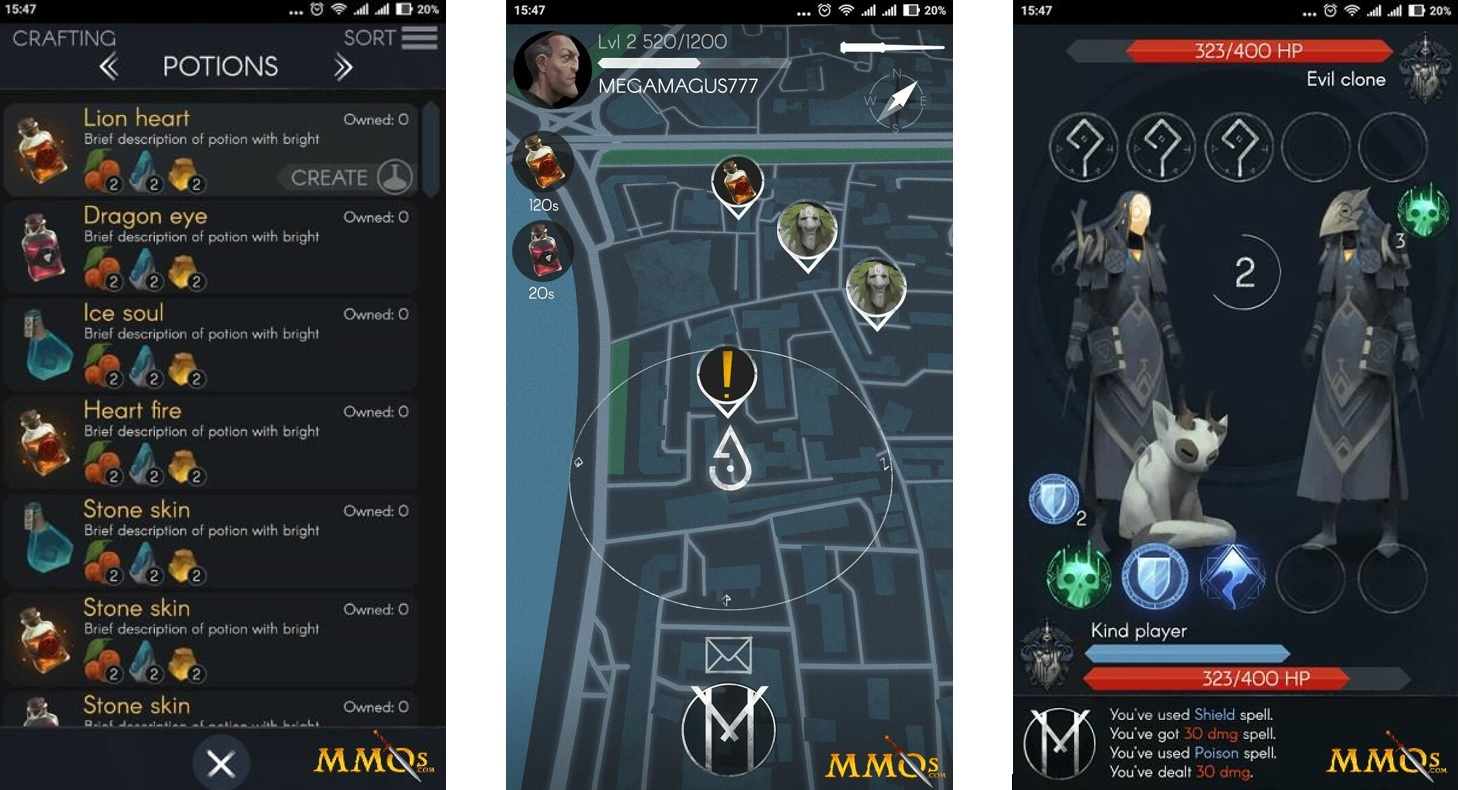
\includegraphics[scale=0.4]{slike/Maguss} \\%veličina u odnosu na širinu linije
			\caption{Prikaz sakupljenih kartica, mape i duela u igrici Maguss}
			\label{fig:Maguss} %label mora biti drugaciji za svaku sliku
		\end{figure}
	
		\textnormal{\textbf{Landlord Real Estate Tycoon} je mobilna igrica u kojoj se prema GPS lokaciji igrača prikazuju stvarne lokacije njemu u blizini u obliku kartica lokacija koje zatim može kupovati. To je prva razlika u odnosu na ovaj projekt, jer će u ovome projektu na jednoj lokaciji biti dostupna samo jedna kartica lokacije te za dobivanje kartice neće biti potrebna nikakva monetarna vrijednost kao što je to u igrici Landlord Real Estate Tycoon. Također se mogu davati ponude za kartice drugih igrača, a cilj igre je istraživanjem, kupovanjem i preprodavanjem povećati svoju monetarnu vrijednost. U igrici Real Estate Tycoon nema ničega sličnog borbama u ovome projektu. Također, u ovome projektu neće biti moguća razmjena kartica između igrača. }
		
		\begin{figure}[H]
			\centering
			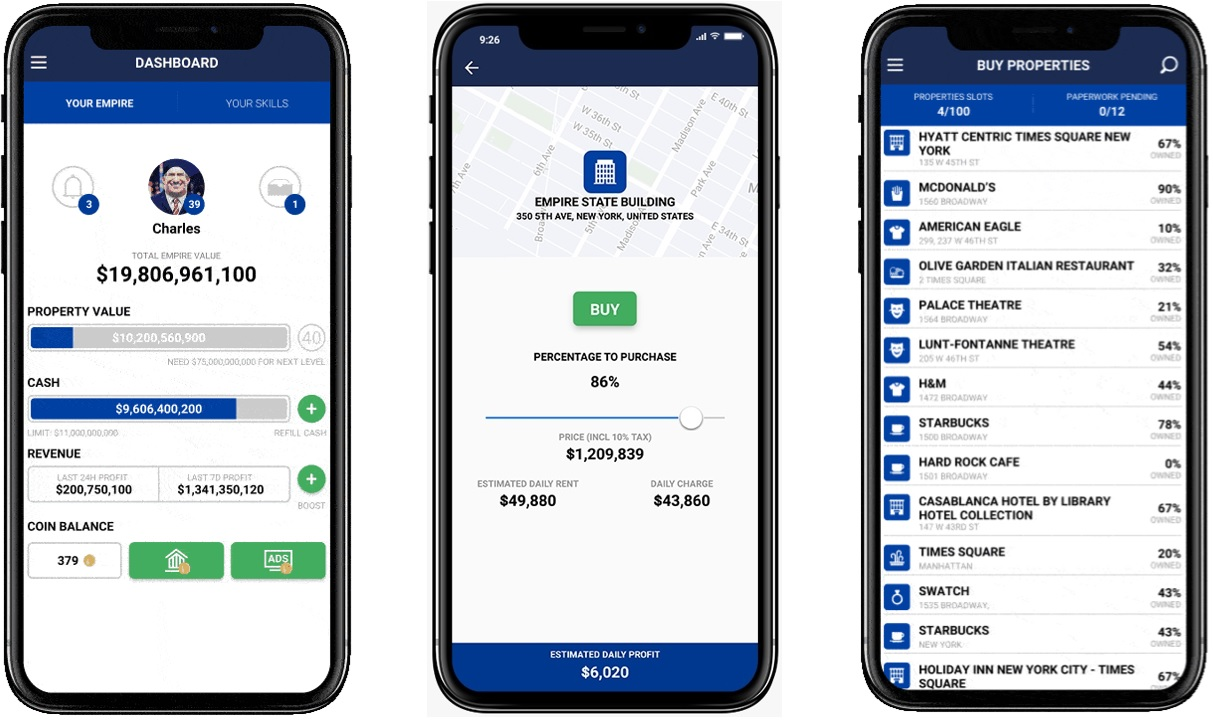
\includegraphics[scale=0.45]{slike/Landlord} \\%veličina u odnosu na širinu linije
			\caption{Prikaz profila igrača, kartice lokacije i dostupnih lokacija u igrici Landlord Real Estate Tycoon}
			\label{fig:Landlord} %label mora biti drugaciji za svaku sliku
		\end{figure}
	
		\textnormal{Još jedna mobilna igrica slična ovome projektu je \textbf{Ghostbusters World}. Igrači trebaju doći na stvarnu lokaciju koja je pomoću GPS-a u igrici označena kao mjesto gdje postoje duhovi. Na tim lokacijama nakon odigrane minigre mogu postaviti zamku te time dobiti nekog od duhova u obliku kartice. Ovo je prva razlika u odnosu na ovaj projekt gdje je sam dolazak na lokaciju dovoljan za dobivanje kartice te je na određenoj lokaciji moguće dobiti isključivo jednu vrstu kartice. Također, u igrici Ghostbusters World omogućen je prikaz duhova u stvarnom svijetu pomoću kamere te prikaz putovanja igrača kroz virtualan svijet, što u ovome projektu neće biti omogućeno. Također su omogućeni dueli igrača gdje se bore sakupljenim karticama duhova, no izbor suparnika ne ovisi o međusobnoj udaljenosti igrača kao što će biti slučaj u ovome projektu, već se igrači smještaju u tzv. Arene, ovisno o napretku u igrici, unutar kojih se mogu boriti.}
		
		\begin{figure}[H]
			\centering
			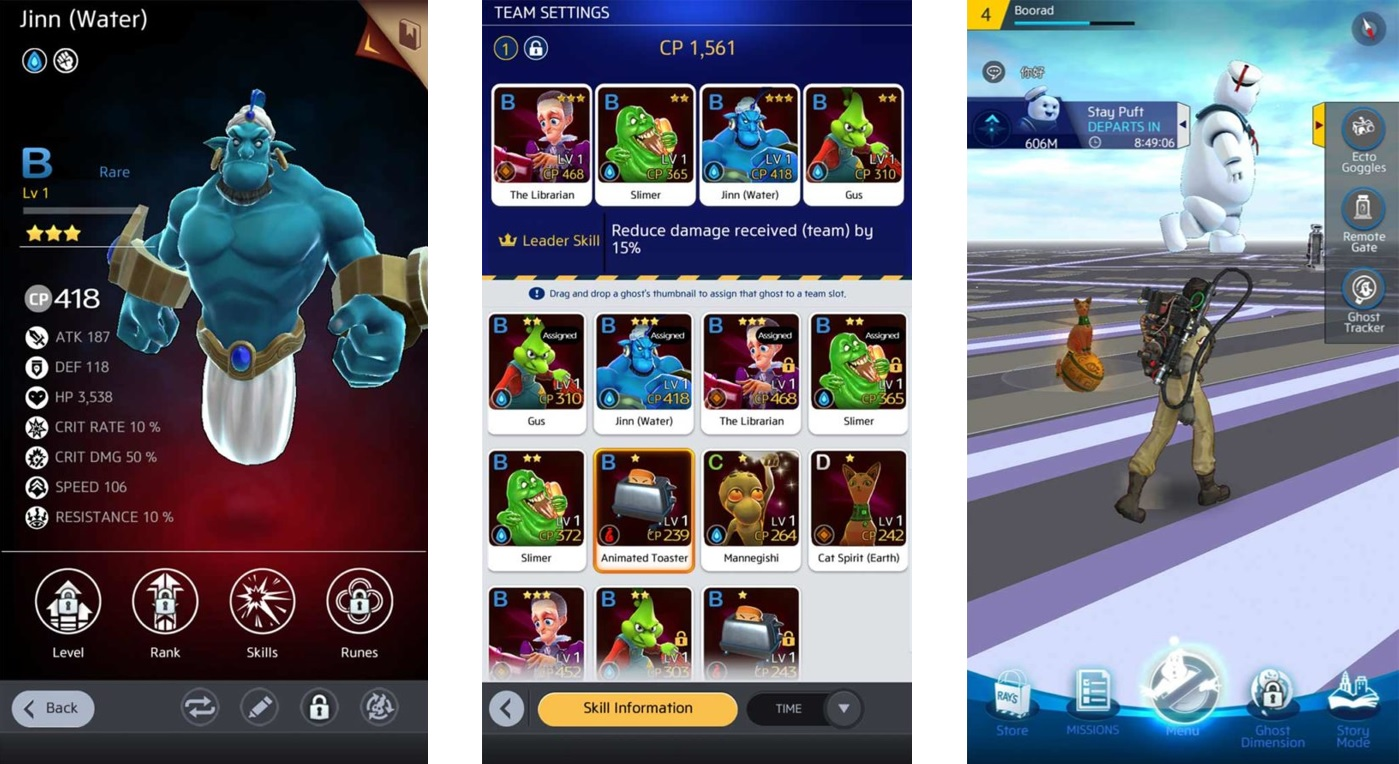
\includegraphics[scale=0.45]{slike/Ghostbusters} \\%veličina u odnosu na širinu linije
			\caption{Prikaz igrače kartice, sakupljenih kartica i igrača virtualnom svijetu igrice Ghostbusters World}
			\label{fig:Ghostbusters} %label mora biti drugaciji za svaku sliku
		\end{figure}	
		
		\textnormal{Ova aplikacija ne mora se nužno koristiti za borbu među igračima. Za ljude koji su avanturisti a ne zanima ih borba i igranje igrice, aplikacija bi se mogla korisnicima služiti kao evidencija mjesta koja su posjetili. Dodavši mogućnost kontaktiranja i razmjenjivanja poruka između avanturista, aplikacija  bi poprimila ugođaj društvene mreže na kojoj bi se ljudi mogli povezati s drugim avanturistima koji su bili na sličnim mjestima/putovanjima. Razmjenjivanjem iskustava i preporuka, stvorila bi se mreža avanturista koji jedni drugima preporučaju zanimljive lokacije i postižu zadane si ciljeve.}
		
		\textnormal{Još jedna mogućnost je prilagođenje aplikacije za korištenje u edukativne svrhe. Prilikom namjernog ili nenamjernog posjeta nekoj obilježenoj lokaciji, osoba bi primila obavijest s informacijama o mjestu koje je posjetila, zajedno sa slikama i linkovima za više informacija. Iste informacije bi mogla naknadno pogledati na svome korisničkom računu, na sučelju s posjećenim mjestima.}\\
		
		\textnormal{Ideja ovog projekta je potaknuti igrače na fizičku aktivnost i na bolje upoznavanje okruženja u kojem žive. Na zabavan način i kroz igru, igrači se potiču na izlazak iz svojih domova i provođenje slobodnog vrijeme hodajući. Nezdrav način igranja igara u foteljama i stolcima, zamijenila je lagan fizička aktivnost. Uz to igračima se daje mogućnost obići njima do sada nepoznate znamenitosti svog mjesta. Lokacije za dobivanje igraćih karata prolaze kroz strogu kontrolu te garantiraju točne i igračima zanimljive informacije. Igrači ujedno mogu i dati prijedlog za novu lokaciju i time sačuvati od zaborava priču koja ih veže za tu lokaciju. Na ovaj način svim posjetiteljima tog mjesta omogućeno je lagano, zabavno i efikasno upoznavanje svih čari mjesta u kojem se nalaze.}\\
		
		\textnormal{Ovisno o uspješnosti projektnog zadatka i dodatnim zahtjevima korisnika moguća je nadogradnja nativna iOS i Android aplikacija kako bi se poboljšale performanse na mobilnim uređajima. Također, integracije s najpopularnijim društvenim mrežama bi se ugradile kako bi igrači podijeliti svoje uspjehe s prijateljima. Uvođenjem sustava achievementa(dostignuća) mogli bi se dodatno nagrađivati igrači za posebne milestone(prekretnice) u igri. Igrači bi mogli vidjeti koje achievemente još nisu osvojili i koji su koraci sve potrebni da ih osvoje. Korištenjem API-ova možemo nadopuniti listu lokacija, te ubrzati postupak njihovog dodavanja. Za vrijeme posebnih događaja kao što su Nova godina, Božić i slično mogli bi dodati posebne karte koje se samo tada, u kratkom roku, mogu skupiti. Uvođenje posebnih lokacija za koje je potrebno više ljudi da se osvoje je također moguća nadogradnja. Najveća potencijalna nadogradnja je uvođenje AR (Augmented reality) sposobnosti kako bi igrači mogli oko sebe pomoću ugrađene kamere na mobilnom uređaju lakše pronaći sve moguće lokacije u svojoj blizini.}
		
		\eject
		
		\section{Primjeri u \LaTeX u}
		
		\textit{Ovo potpoglavlje izbrisati.}\\

		U nastavku se nalaze različiti primjeri kako koristiti osnovne funkcionalnosti \LaTeX a koje su potrebne za izradu dokumentacije. Za dodatnu pomoć obratiti se asistentu na projektu ili potražiti upute na sljedećim web sjedištima:
		\begin{itemize}
			\item Upute za izradu diplomskog rada u \LaTeX u - \url{https://www.fer.unizg.hr/_download/repository/LaTeX-upute.pdf}
			\item \LaTeX\ projekt - \url{https://www.latex-project.org/help/}
			\item StackExchange za Tex - \url{https://tex.stackexchange.com/}\\
		
		\end{itemize} 	


		
		\noindent \underbar{podcrtani tekst}, \textbf{podebljani tekst}, 	\textit{nagnuti tekst}\\
		\noindent \normalsize primjer \large primjer \Large primjer \LARGE {primjer} \huge {primjer} \Huge primjer \normalsize
				
		\begin{packed_item}
			
			\item  primjer
			\item  primjer
			\item  primjer
			\item[] \begin{packed_enum}
				\item primjer
				\item[] \begin{packed_enum}
					\item[1.a] primjer
					\item[b] primjer
				\end{packed_enum}
				\item primjer
			\end{packed_enum}
			
		\end{packed_item}
		
		\noindent primjer url-a: \url{https://www.fer.unizg.hr/predmet/proinz/projekt}
		
		\noindent posebni znakovi: \# \$ \% \& \{ \} \_ 
		$|$ $<$ $>$ 
		\^{} 
		\~{} 
		$\backslash$ 
		
		\begin{longtabu} to \textwidth {|X[8, l]|X[8, l]|X[16, l]|} %definicija širine tablice, širine stupaca i poravnanje
			
			%definicija naslova tablice
			\hline \multicolumn{3}{|c|}{\textbf{naslov unutar tablice}}	 \\[3pt] \hline
			\endfirsthead
			
			%definicija naslova tablice prilikom prijeloma
			\hline \multicolumn{3}{|c|}{\textbf{naslov unutar tablice}}	 \\[3pt] \hline
			\endhead
			
			\hline 
			\endlastfoot
			
			\rowcolor{LightGreen}IDKorisnik & INT	&  	Lorem ipsum dolor sit amet, consectetur adipiscing elit, sed do eiusmod  	\\ \hline
			korisnickoIme	& VARCHAR &   	\\ \hline 
			email & VARCHAR &   \\ \hline 
			ime & VARCHAR	&  		\\ \hline 
			\cellcolor{LightBlue} primjer	& VARCHAR &   	\\ \hline 
			
		\end{longtabu}
		

		\begin{table}[H]
			
			\begin{longtabu} to \textwidth {|X[8, l]|X[8, l]|X[16, l]|} 
				
				\hline 
				\endfirsthead
				
				\hline 
				\endhead
				
				\hline 
				\endlastfoot
				
				\rowcolor{LightGreen}IDKorisnik & INT	&  	Lorem ipsum dolor sit amet, consectetur adipiscing elit, sed do eiusmod  	\\ \hline
				korisnickoIme	& VARCHAR &   	\\ \hline 
				email & VARCHAR &   \\ \hline 
				ime & VARCHAR	&  		\\ \hline 
				\cellcolor{LightBlue} primjer	& VARCHAR &   	\\ \hline 
				
				
			\end{longtabu}
	
			\caption{\label{tab:referencatablica} Naslov ispod tablice.}
		\end{table}
		
		
		%unos slike
		\begin{figure}[H]
			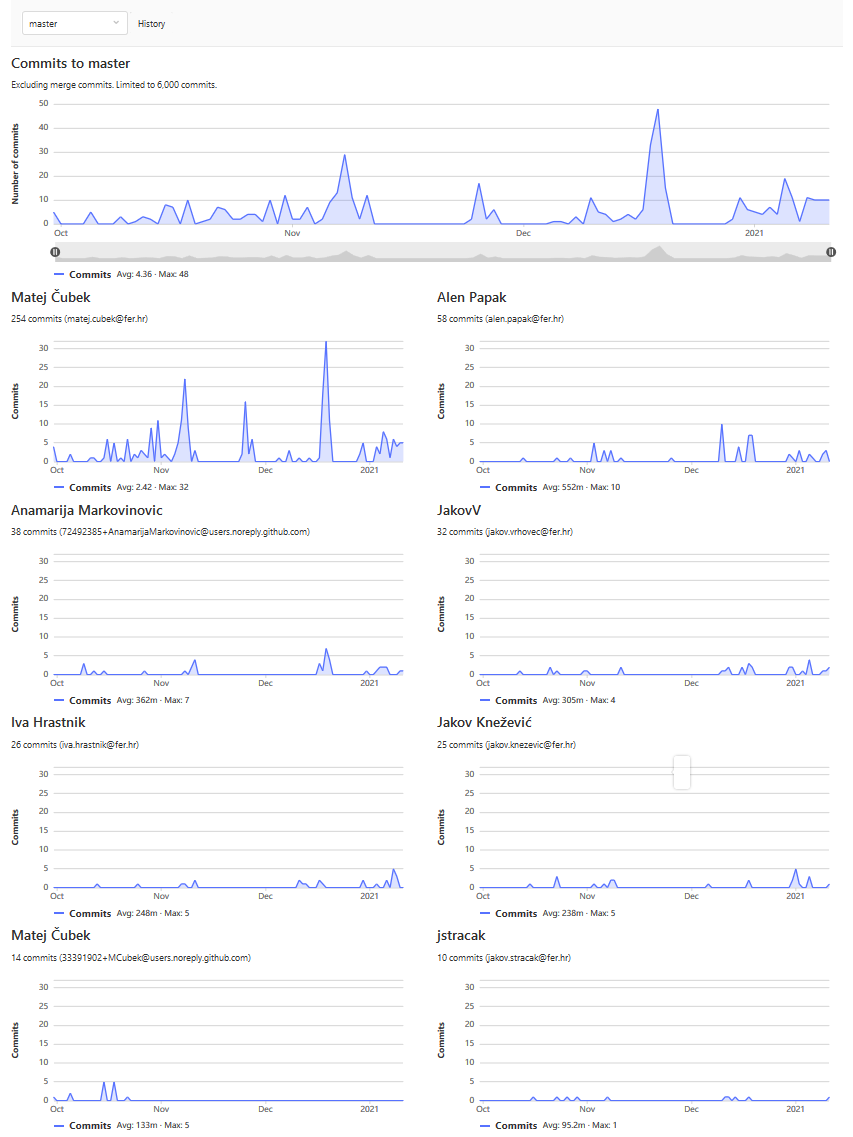
\includegraphics[scale=0.4]{slike/aktivnost.PNG} %veličina slike u odnosu na originalnu datoteku i pozicija slike
			\centering
			\caption{Primjer slike s potpisom}
			\label{fig:promjene}
		\end{figure}
		
		\begin{figure}[H]
			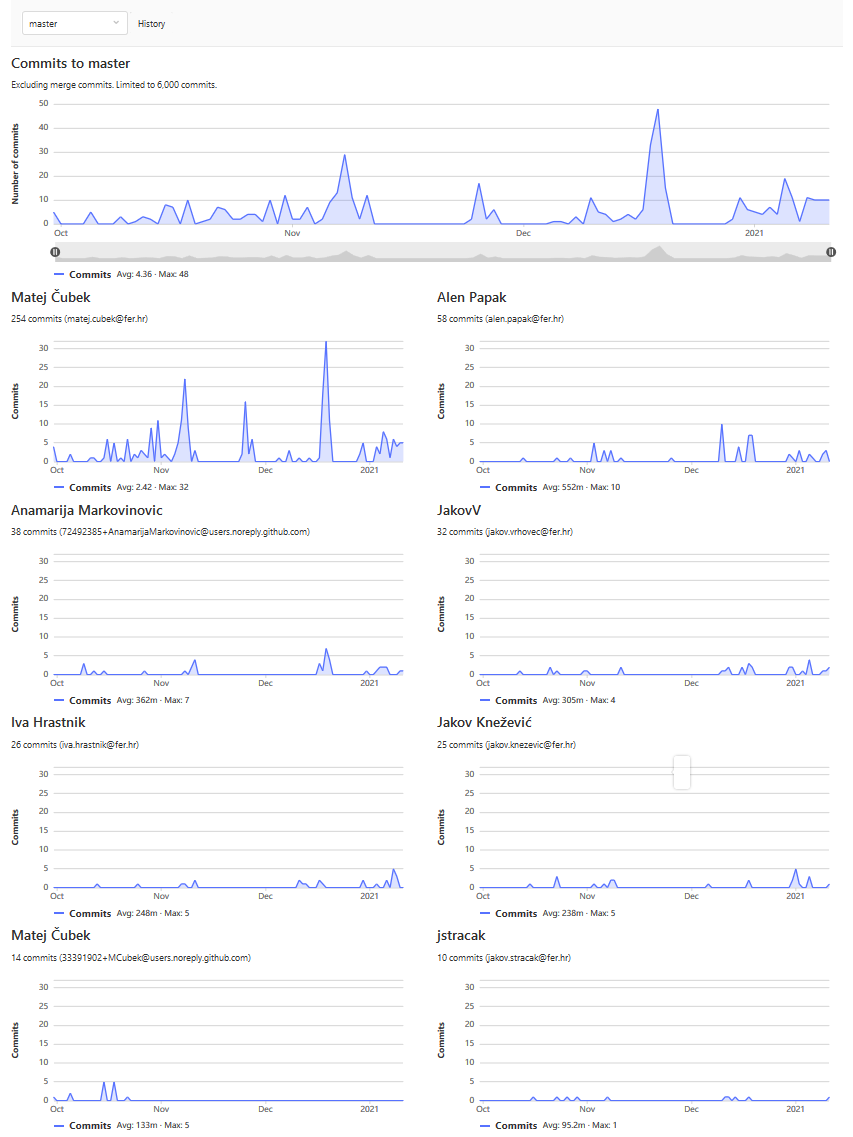
\includegraphics[width=.9\linewidth]{slike/aktivnost.PNG} %veličina u odnosu na širinu linije
			\caption{Primjer slike s potpisom 2}
			\label{fig:promjene2} %label mora biti drugaciji za svaku sliku
		\end{figure}
		
		Referenciranje slike \ref{fig:promjene2} u tekstu.
		
		\eject